\section{Implementation}\label{impl}

\begin{figure}[t]
%\vspace{0.2in}
\centering
%\resizebox{0.7\linewidth}{!}{
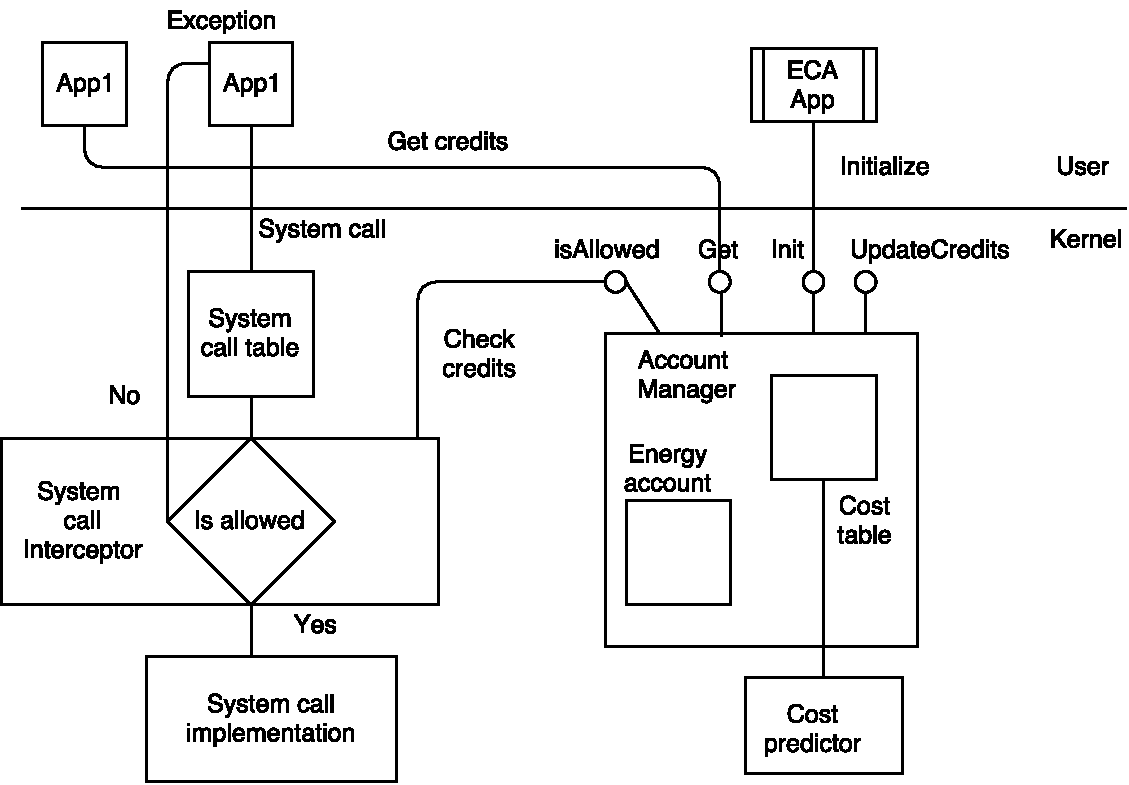
\includegraphics[width=0.8\linewidth]{Figs/mobileapp}
%}
\caption{Architecture.}
\label{fig:Architecture}
\centering
\end{figure}


\subsection{Technical Approach}

Our EnergyMAC framework (see Fig ~\ref{fig:Architecture}) comprises of four components:

\begin{enumerate}

\item Energy Credits allocation System App (ECA app): is a system app that facilitates user to see and allocate priorities for user apps installed in the mobile device. When a user allocates the priorities for apps, ECA app invokes the system call of Energy Accounting Manager in android kernel to save the app details and designated credits.

\item System Call Interceptor: is a component that intercepts the system calls from apps and consults Energy Accounting Manager to check credits that will be spent for that System Call and credits remaining for the app. If the enough energy credit is available, then it redirects to the actual system call else custom exception is thrown stating that required energy credits are not available for that operation.

\item Energy Accounting Manager: Two hash tables for storing records related to app's priority, assigned credits, and each System call's estimated cost (constant cost) are created in the Kernel. One table i.e. Energy account, is used for storing the app UID, priority and assigned credits and another table named Cost sheet is used for storing System call info and corresponding constant cost in terms of credits. Energy account will be refilled with credits at the end of each time period using a Linux kernel timer.

Energy Accounting Manager has access to above tables and exposes APIs for various operations:

\begin{itemize}
\item Get priority and length of time period for app/s
\item Update priority for app/s
\item Get cost of system call
\item Update cost of system call
\item Check if a given system call is allowed
\end{itemize}


\item System Call Price Manager: initializes cost table with cost for all system calls that have constant cost. Moreover, it will also estimate cost of variable cost system calls using models. These models will be derived from previous work such as Eprof.


\end{enumerate}

\subsection{How it works}

Android OS is divided between User Space and Kernel Space based on the type of actions that can be performed by user program and OS itself. This separation is required to provide isolation and abstraction. The Kernel has the privileges for managing the system resources and User programs do not. So, user program communicate with Kernel via system call to use services provided by OS. 

Each system call is represented by a number in system call table in the kernel. Since apps in the user space invoke system call for different operations, this system call can be intercepted and decision can be taken whether the system call should be executed. This is the basis for enforcing the energy accounting policies on apps in our energy accounting system. 

In Energy accounting system, the user allocates the available priorities for the apps that user intends to use via ECA App. This internally invokes the custom system calls that are part of Energy Accounting Manager, to update the priority of the apps and data is stored in the Energy account hash table. The accounting system had a kernel timer which times out at the end of each time period and credits will be updated in Energy account hash-table based on the priority of the app for next time period. 

The cost of each system call in terms of energy credits is decided by the System Call Price Manager depending upon the energy model for that system call and constant costs will be stored in the hash table named Cost sheet. 

When an app, in this case, GPS App, tries to use get the location, then it invokes the system call to get the location of the device. At this time, the system call is intercepted by the Interceptor and it checks with the Energy Accounting Manager if an app has enough credits to actually invoke that system call related to GPS. If the app has credits more than required to invoke the system call, then the Interceptor redirects to the actual system call and the corresponding credits for that system call is deducted from the allocated credits for that app. Otherwise, the custom exception is thrown back to the application stating that not enough credit is available for that operation and app has to adapt itself accordingly. 

The app can also check whether the operation is permitted and also time period with Energy Accounting Manager and change App's behavior accordingly. 



\subsection{Implementation choices}

There are mainly 5 different layers in Android OS i.e. System Apps, Java API framework, Native Libraries and Android Run time, Hardware Abstraction Layer and Linux Kernel. The Energy Accounting system could have been part of any layer but the decision to make it part of Kernel for the following reasons:

\begin{enumerate}

\item The operations will be protected: The malicious apps will not be able to steal the energy credits or change priority of other benign apps. Only System app and kernel components will have access to the system call related to energy credits update APIs.

\item If it were pushed to any layer above kernel, that would have involved changes in multiple components in that layer and it would not have been easily extendibles for future changes. The kernel is the centralized place to receive all the system calls and due this the changes required in one place and less invasive. For example if this energy accounting were to be moved to the Java API framework level, closer to the layer where app reside, then the changes had to be done in multiple components like Location Manager, Telephony manager,etc in this layer and that would have been more invasive.

\item Previous work such as Eprof has models for calculating energy costs of system calls. 

\end{enumerate}

Following changes were made in OS Kernel as part of the implementation:

\begin{enumerate}

\item System calls and their implementation corresponding to the APIs of the Energy Accounting Manager were added to the Kernel.
\item Two hash tables were created in the kernel memory to store energy accounting related information.
\item The system call number of the socket system call i.e. sys\_socket was replaced by the system call number of the Interceptor in the system call table in the kernel.

\end{enumerate}



